%Chapter of Implementation
%What my app has, (how it evolved?) in terms of physical structure and technologies involved

\chapter{Implementation}
\label{imple}

\section{Overview}

The Arduino Due asks for the server's new public key and for a new nonce that it should use for the following temperature data transmission. It does this by sending a GET request to a JSP page on the server. The public key and nonce are newly generated by the server and the nonce is sent securely. The Due is connected to the DS18S20 temperature sensor and it receives the temperature data over the OneWire protocol. This data is signed using the Arduino's private signature key and then encrypted using the Arduino's private key, the Server's new public key and the new nonce. The encrypted data is sent as a POST request to the add.php file on the apache server which executes the file and the first thing add.php does is call connect.php which has the SQL database details and makes a connection to the database. Following that add.php builds up a SQL query that inserts the values sent in the post request into the appropriate table entries and then the connection is closed.
When a user want to view the files, they use a browser to send a GET request to the Java web app. The app builds up a SQL query to take out all the values from the database, decrypts them and verifies the signature before printing out in a table.
When it comes to public key transmission the Due sends a POST request to the Arduino Uno that is set up as a web server. The Uno recognises that it is receiving a POST request and stores the key. A visual representation of these steps can be seen in figure \ref{fig:messeq}.




\begin{figure}[H]
 % \centering
\begin {sequencediagram}

	\newthread[blue]{due}{: Arduino Due }
	\tikzstyle{inststyle}+=[bottom color=babyblueeyes]
	\newinst [1]{server}{: WebServer}
	\newinst {ds}{: DS18S20 Sensor }
	\newinst {uno}{: Arduino Uno }
	
	\begin {call}{due}{GET request}{server}{Key/Nonce}
	\end {call}
	%\begin {sdblock}{ Run Loop }{ The main loop }
	\begin {call}{due}{ GetTemp}{ds}{}
	%\begin {call}{ctr}{ ActAgent () }{sense}{}
	%\end {call}
	\end {call}
	\begin {call}{due}{ SendSecureTemp}{server}{}
	%\begin {messcall}{ps}{ PrePhysicsUpdate () }{sense}{state}
	%\end {messcall}
	%\begin {sdblock}{ Physics Loop }{}
	%\begin {callself}{ps}{ PhysicsUpdate () }{}
	%\end {callself}
	%\end {sdblock}
	\end {call}
	\begin {call}{due}{ SendPublicKey}{uno}{}
	
	\end {call}
	%\begin {call}{ss}{ EndCycle () }{ctr}{}
	%\begin {call}{ctr}{ SenseAgent () }{sense}{}
	%\end {call}
	%\end {call}
	%\end {sdblock}
\end {sequencediagram}
  \caption{System sequence diagram}
  \label{fig:messeq}
\end{figure}

\subsection{Temperature reading}

The DS18S20 temperature sensor is wired up with a 4.7$\Omega$ pull up resistor, between the orange wires, on the bread board shown in figure \ref{fig:tempcircuit}. A pull up resistor is a resistor between the sensor and the positive power supply so that the signal will be a valid logic level if external devices are disconnected or a high impedance is introduced. It is connected to digital pin 9, yellow wire, because it can't be on pins 10, 11, 12, 13 as they will be used by the Ethernet Shield. When looking at the temperature sensor the furtherest left pin is V$_{dd}$ and normally this would be connected to the Arduino's 3.5v or 5v output but the DS18S20 is in parasite power mode which scavenges power off the middle data line, DQ. When the DQ pin is high some of the charge is stored in a capacitor that will be used to power the device when the data is being read. In parasite power mode both the GND and V$_{dd}$ are connected together, by the bluewire, and then to ground. The circuit diagram shown was created with Fritzing \cite{fritz}.

\begin{figure}[H]
	\centering
	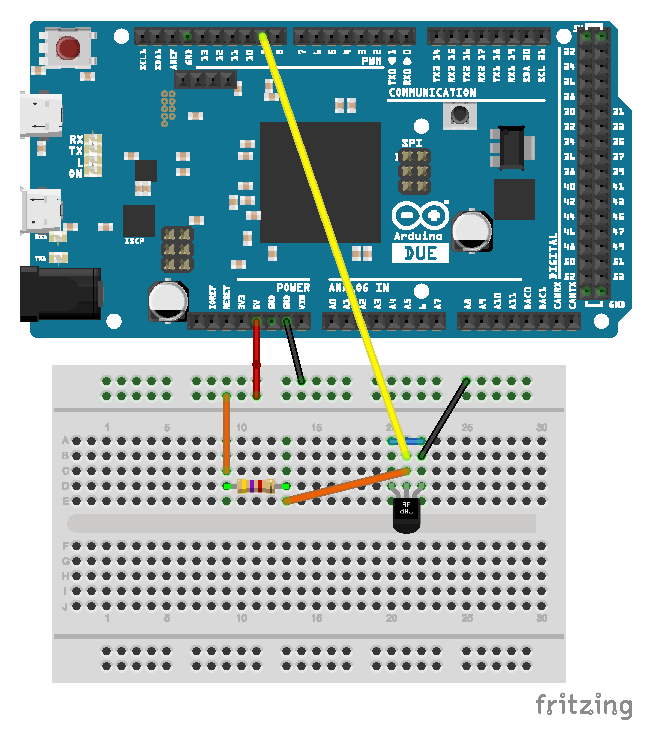
\includegraphics[width=.5\linewidth]{Figures/TempSensor_bb.pdf}
	\caption{DS18S20 in parasitic power mode connected to Arduino}
	\label{fig:tempcircuit}
\end{figure}

%can explain full scratchpad memory, CRC, or hex to int conversion
The DS18S20's scratchpad memory is divided up into 9 bytes as shown in figure \ref{fig:dsmem}. The first two bytes are the ones of most interest as they store the actual temperature value. Bytes 2 and 3 are the high and low trigger registers, these can be used to trigger some action when the temperature goes above or below a certain threshold. Bytes 4 and 5 are only for internal use and cannot be overwritten. Bytes 6 and 7 can be used to calculate the extended resolution. Byte 8 holds the cyclic redundancy check which is an error detecting technique. The bytes with asterisks are values which stored in non volatile EEPROM, the rest are stored on volatile SRAM. The shown table was taken from the DS18S20 datasheet \cite{dsdatasheet}.

\begin{figure}[H]
	\centering
	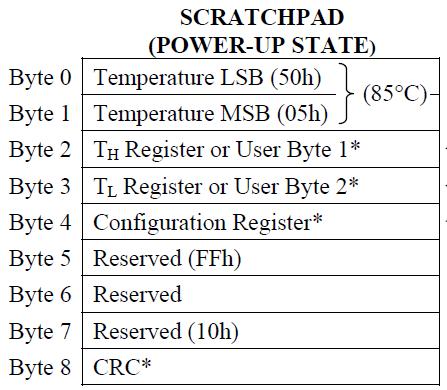
\includegraphics[width=.6\linewidth]{Figures/dsmem.png}
	\caption{DS18S20's memory organisation}
	\label{fig:dsmem}
\end{figure}

The library used to read the DS18S20 is OneWire, which is a proprietary library from Maxim that performs half-duplex bidirectional communications between a host/master controller and one or more slaves. As seen in the following code snippet, figure \ref{snip:tempcode}. The command \emph{ds.write(0x44, 1)} starts the internal A-D conversion operation. Once this process is finished the data is copied to the Scratchpad registers. A delay is needed to charge the capacitor and to ensure conversion is complete before reading the data. Which is done with \emph{ds.write(0xBE)} and then the data is read out using \emph{ds.read()} and put into an array.

\begin{figure}[H]
\begin{lstlisting}[style=Arduino]
  							OneWire  ds(9);
								...
  							ds.write(0x44, 1); 
  						 	delay(1000);

  							present = ds.reset();
  							ds.select(addr);    
 							ds.write(0xBE)

  							Serial.print("  Data = "); 
  							Serial.print(present, HEX);
 						 	Serial.print(" ");
  							for ( i = 0; i < 9; i++) {          
    								data[i] = ds.read();
    								Serial.print(data[i], HEX);
    								Serial.print(" ");
  							}

\end{lstlisting}
\caption{DS18S20 temperature sensor Arduino Code}
\label{snip:tempcode}
\end{figure}


\section{Security}

Before the data can be signed and authenticated encrypted the new nonce and server public key have to be requested. The Due sends, to the server, a GET request in a very similar manner to the POST request shown in figure \ref{snip:ethernet} and the server returns, byte by byte, the information. The POST request is sent to a JSP page called Secret Key. So called because it updates the Server's authenticated encryption key pair and not because it sends the private key anywhere. It's implementation is described in section \ref{pktransmit}. The Arduino takes the char arrays and converts them into two different byte arrays, one for the nonce and one for the public key. The public key is sent unencrypted but as a proof of concept the nonce is sent authenticated encrypted and signed. This is to show that with pre-installed keys it possible to update the keys and other data securely and then use the updated information to facilitate further information updates. Generally the nonce and public keys are sent unencrypted when it is a first transmission as there is no other way. Shown in figure \ref{snip:denonce} is the code to decrypt the nonce, if this is the first transmission then the nonce will have been encrypted with the pre-installed keys and nonce, else the server public key and nonce generated by the server for the previous secure temperature data transfer are used. The decision process is shown in figure \ref{snip:noncedec}. 

The way the Arduino Due knows if this is the first transmission is if the byte array \emph{serverpkold} is empty, as after the temperature data is encrypted with this new nonce and server public key they become the old nonce and server public key. After becoming the old nonce and server public key they are stored in different arrays so they can be used to decrypt the next nonce as the next nonce from the server will be encrypted using the private key that is mathetically linked to this ``old'' server public key and nonce.

  The keys used for the signature process and the set used for the authenticated encryption process are not the same. There are four key pairs used in this prototype. A key pair is a set of one public key and one private key. The Arduino Due has a signature key pair and an authenticated encryption key pair. The web server, also, has a signature key pair and an authenticated encryption key pair. The signature key pairs stay the same through out the application, so does the Arduino Due's authenticated encryption key pair. Of the keys, it is only the Server's authenticated encryption key pair that is updated.
The Due decrypts the nonce using the relevant keys and removes the 32 bytes of leading zeros that needed to be placed by the server for successful encryption before verifying the signature in line 19 of figure \ref{snip:denonce}. Nonces are 24 bytes in length and a signature is 64 bytes in length.

It is a bit unusual to update the server's public key so regularly. Normally there would be huge gaps of time between key updates because if the cryptographic library being used is good then it should take a long time to break. However sometimes keys become compromised and need to be changed so to highlight and demonstrate how keys could be updated, the server's keys were updated for each message.

\begin{figure}[H]
\centering
\begin{tikzpicture}[node distance = 4cm, auto]
    % Place nodes
    \node [decision] (decidekey) {Is this the first transmission?};
    \node[input, left of=decidekey](yes){Yes};
    \node[input, right of=decidekey](no){No};
    \node [blockf, below of=yes, node distance=3cm](seryes){Server: Encrypt Nonce with pre-installed keys};
    \node [blockf, below of=no, node distance=3cm](serno){Server: Encrypt Nonce with previous keys};
    \node[blockf, below of=seryes](dueyes){Due: Decrypt Nonce with pre-installed keys};
    \node[blockf, below of=serno](dueno){Due: Decrypt Nonce with previous keys};
    % \node [blockf] (init) {initialize model};
    %\node [cloud, left of=init] (expert) {expert};
    %\node [cloud, right of=init] (system) {system};
    %\node [blockf, below of=init] (identify) {identify candidate models};
    %\node [blockf, below of=identify] (evaluate) {evaluate candidate models};
    %\node [blockf, left of=evaluate, node distance=3cm] (update) {update model};
    
    %\node [blockf, below of=decide, node distance=3cm] (stop) {stop};
    % Draw edges
    \path [line] (decidekey) -| node [near end]{Yes} (seryes);
    \path [line] (decidekey) -| node [near end] {No}(serno);
    %\path [line] (yes) -- (seryes);
    \path [line] (no) -- (serno);
    \path [line] (seryes) -- (dueyes);
    \path [line] (serno) -- (dueno);
    %\path [line] (decide) -| node [near start] {yes} (update);
    %\path [line] (update) |- (identify);
    %\path [line] (decide) -- node {no}(stop);
    %\path [line,dashed] (expert) -- (init);
    %\path [line,dashed] (system) -- (init);
    %\path [line,dashed] (system) |- (evaluate);
\end{tikzpicture}
\caption{Nonce Decision Tree}
\label{snip:noncedec}
\end{figure}


\begin{figure}[H]
\begin{lstlisting}[style=Arduino]
#include <TweetNaCl2.h>
TweetNaCl2 tnacl;
int Suc_Decrypt;
int Suc_SignVerify;
int scnlenwz = crypto_box_NONCEBYTES + crypto_sign_BYTES + crypto_box_ZEROBYTES; 
byte scnoncenewtemp[scnlenwz]; //signed encrypted nonce with zeros
byte snoncewz[scnlenwz]; // signed nonce with zeros
int snlenwoz = crypto_box_NONCEBYTES + crypto_sign_BYTES;
byte snoncewoz[snlenwoz]; //signed nonce without zeros
int snlen = crypto_box_NONCEBYTES;
byte nonce[snlen];
	...
if(serverpkold[0]==NULL){
	Suc_Decrypt = tuit.crypto_box_open(snoncewz, scnoncenewtemp, scnlenwz, preinstallnonce, preinstallserverpk, arduinosk); 
}else{
	Suc_Decrypt = tuit.crypto_box_open(snoncewz, scnoncenewtemp, scnlenwz, nonceold, serverpkold, arduinosk);
}

Suc_SignVerify = tuit.crypto_sign_open(nonce,&nlen,snoncewoz,snlenwoz,serverpksign);

\end{lstlisting}
\caption{Decrypting the next nonce}
\label{snip:denonce}
\end{figure}

Now that the server public key and nonce have been found the secure temperature data transmission can take place. Much like the server, when the Arduino is encrypting a signature and message it must have padded out the data with 32 bytes of leading zeros specified in the NaCl website. Take special care that exactly 32 bytes are placed in front because if there isn't the correct number the encryption process will still complete without errors. However the decryption will fail and it isn't apparent that that error occurred when data was encrypted. The code used to sign and encrypt the data is shown in figure \ref{snip:nacl}.

It is a little unusual to employ both authenticated encryption and a signature process. This was done to show off more of the capabilities of the TweetNaCl library and to provide an extra layer of authenticity as an attacker would need another key pair to fully exploit the message.

\begin{figure}[H]
\begin{lstlisting}[style=Arduino]
#include <TweetNaCl2.h>
TweetNaCl2 tnacl;

byte arduinosk[crypto_box_SECRETKEYBYTES] = {...};
byte arduinosksign[crypto_sign_SECRETKEYBYTES] = {...};
byte serverpk[crypto_box_PUBLICKEYBYTES]  = {...};
byte nonce[crypto_box_NONCEBYTES] = {...};

int const messageLength = crypto_sign_BYTES + 9;
byte message[messageLength] = {...};
unsigned long long signedMessageLength=0;
byte signedCipher[signedMessageLength];
unsigned char signedMessage[messageLength+crypto_sign_BYTES];

tnacl.crypto_sign(signedMessage, &signedMessageLength, message, messageLength, arduinosksign);
tnacl.crypto_box(signedCipher, signedMessage, signedMessageLength, nonce, serverpk, arduinosk);
\end{lstlisting}
\caption{TweetNaCl Arduino Signature and Encryption Code}
\label{snip:nacl}
\end{figure}

The C TweetNaCl library has been converted into an Arduino library. It therefore needs an instance of TweetNaCl created which in the sketch is called \emph{tnacl}. With this instance the methods needed can be accessed. In this prototype some keys are preinstalled, the Arduino's authenticated encryption key pair, it's signature key pair, the server's signature key pair and the first nonce and first server authenticated encryption key pair that will only be used once to decrypt the first nonce. With each transmission the server's authenticated encryption key pair is updated and the Due will get a new nonce and server public key. 

Lines 4-13 set up the message byte arrays that are to be passed between the methods. \emph{message} is initialised as a byte array of size \emph{messageLength} which is \emph{crypto\_box\_ZEROBYTES}, 32 bytes, plus the length of the message. The first byte of the message contains the Arduino's unique identifier to prove the Arduino was the original sender and the second byte contains the server's unique identifier to prove that the message was meant for the server. \emph{signedMessage} and \emph{signedMessageLength} are passed in by reference so after \emph{crypto\_sign()} is complete the message with the signature and the size of that array will be in those variables, respectively. The resulting signed message needs to have 32 bytes of leading zeros added to it before encryption. The function \emph{crypto\_box} completes the authenticated encryption and places the cipher into \emph{signedCipher} which is passed in by reference. 

\clearpage

\section{Data transmission}
Once the data has been encrypted it is to be packaged up and sent across the network.

\begin{figure}[H]
\begin{lstlisting}[style=Arduino]
#include<Ethernet2.h> //Ethernet Shield R2 library
#include<SPI.h>

byte mac[] = {
0x90, 0xA2, 0xDA, 0x10, 0x2D, 0xD6 }; //MAC address of the Ethernet Shield
char server[] = "192.168.0.6"; //IP of apache web server
EthernetClient client;
IPAddress clientIP(192, 168, 0, 30);

 if(Ethernet.begin(mac)==0){
      Serial.println("Failed to assign IP");
      Ethernet.begin(mac, clientIP);
  }else{
     Serial.println("Assigned IP");
  }
if(client.connect(server,80)){
     String data = "temperatureHex=";
     int contentLength = data.length()+final.length();
     Serial.println("Connected");   
     client.println("POST /tempLog/add.php HTTP/1.1"); 
     client.println("HOST: 192.168.0.6"); 
     client.println("Content-Type: application/x-www-form-urlencoded");
     client.print("Content-Length: ");
     client.println(contentLength);
     client.println();
     client.print("temperatureHex=");
     client.print(final);
   }else{
       Serial.println("Failed to Connect");
   }
   client.stop();
\end{lstlisting}
\caption{Ethernet interfacing and transmission Code }
\label{snip:ethernet}
\end{figure}

 Just before the cipher is sent the byte array is converted into a String so that it can be passed around easily as one parameter. This is completed simply by cycling through the byte array and adding each entry together. Care has to be taken when there are hexadecimals that are 0x0F or lower. The leading zero is lost during the conversion to String which means that when the cipher reconverted into a byte array, it is incorrect and cannot be decrypted. This is solved by explicitly adding an extra ``'0'' String if the byte is less than or equal to 0x0F. The Arduino Due needs to know the MAC address of the Ethernet shield if it is to make contact with the server. A media access control address, MAC is a unique identifier assigned to network interfaces. It allows the router to know what device the data is being sent from and where to send the replies. It is not dynamic. The device now needs an IP address which is completed through the Dynamic Host Configuration Protocol, DHCP, by the router. The router running DHCP dynamically allocates network configuration parameters such as IP addresses to devices so that they automatically get one that isn't in use. This is completed with the line \emph{Ethernet.begin(mac)} on line 10 in figure \ref{snip:ethernet} which returns a 1 on successful IP allocation or 0 on failure. If it fails then a static IP can be assigned manually by \emph{Ethernet.Begin(mac, clientIP)}. A connection to the server is attempted using the IP and the port number, 80 in this case. It is worth mentioning here, if the server is running on a Windows OS then make an exception for the IP address of the Arduino Due otherwise Windows firewall will block it. If it successful the information is transmitted as a POST request, a POST request is a request method in the HTTP protocol. When a server receives a POST request it knows to take the data and complete an action with it. The request makes it known that it wants add.php to be executed upon receiving the data. %extra params, the content size and urlencoding
Once the data is sent the connection can be closed and other actions performed on the Arduino.
 
\section{Server Side}

For the prototype, an Apache and Tomcat server with SQL was set up using XAMPP on a desktop. The Arduino Due causes the add.php to be run and the first thing that add does is call connect.php that creates a connection to the relational database using SQL's IP address, username, password and the name of the database. If it can't connect it abandons the task and returns an error message. On successful connect it returns the connection variable.

\begin{figure}[H]
%\begin{lstlisting}[language=PHP]
\begin{lstlisting}[style=PHP]
<?php
   	include("connect.php");
 
   	$link=Connection();
	
	$temp=$_POST["temperatureHex"];
 
	$query = "INSERT INTO tempLog (tempHex) 
		VALUE ('".$temp."')"; 
 
   	mysql_query($query,$link);
   	mysql_close($link);
 
   	header("Location: index.php");
?>
\end{lstlisting}
\caption{Arduino to SQL interfacing code}
\label{snip:php}
\end{figure}

After connecting, control is handed back to the add file where the data to be stored is extracted out of the POST request and placed in a variable. Then an SQL query to insert the variable into the correct table is built up before being sent to the SQL server and the connection terminated. The SQL table contains an ID, the time at which the temperature data was received and the data and is created using the command shown in figure \ref{snip:sql}. Note between the database creation code and the PHP file the corresponding variables, tempLog, the table name and tempHex, the data.

\begin{figure}[H]
\begin{lstlisting}[style=SQL]
CREATE TABLE `iotplatform`.`tempLog` ( `id` INT(255) NOT NULL AUTO_INCREMENT , `timeStamp` TIMESTAMP on update CURRENT_TIMESTAMP NOT NULL DEFAULT CURRENT_TIMESTAMP , `tempHex` VARCHAR(100) NOT NULL , PRIMARY KEY (`id`)) ENGINE = InnoDB;
\end{lstlisting}
\caption{SQL database creation code}
\label{snip:sql}
\end{figure}
%InnoDB?


\subsection{Decryption and Temperature Data Display}
\label{decryptemp}

The data stored in the database is still encrypted, now a way is needed to decrypt it and display it to the user. A Java web app, using Java server pages, JSP, was created as there are Java implementations of the TweetNaCl library, among other variations, available\cite{ian}. Eclipse JEE Mars was used to create a dynamic web project which extends HttpServlet for the creation of dynamic web pages. In this you override at least one of the following methods, doGet, doPost, doPut and doDelete. Therefore depending on the type of HTTP request received a different action will occur. This application has the code in the doGet as the server will receive a get request when it is accessed by a user.

\begin{figure}[H]
\begin{lstlisting}[style=Java]
protected void doGet(HttpServletRequest request, HttpServletResponse response) throws ServletException, IOException {
response.setContentType("text/html");
PrintWriter printWriter  = response.getWriter();
printWriter.println("<html>");
}
\end{lstlisting}
\caption{Prepping the client printer in JSP}
\label{snip:clientprinterjsp}
\end{figure}

Using the code shown in figure \ref{snip:clientprinterjsp} the headers and tags you would need and expect in a HTML page can now be printed dynamically much like printing to a console. The keys are defined similarly to the code on the Arduino except the server has it's own secret key and the Arduino's public key.

\begin{figure}[H]
\begin{lstlisting}[style=Java]
	final String DB_URL="jdbc:mysql://localhost/iotplatform";
	String user = "root"; 
	String password = "";
	try
	        {
	          // Register JDBC driver
	          Class.forName("com.mysql.jdbc.Driver").newInstance();

	            // Open a connection
	            Connection conn = DriverManager.getConnection(DB_URL, user, password);

	            // Execute SQL query
	            Statement stmt = conn.createStatement();
	            String sql;
	            sql = "SELECT id, timeStamp, tempHex FROM tempLog";
	            ResultSet rs = stmt.executeQuery(sql);
	            // Extract data from result set
	            while(rs.next()){
	               //Retrieve by column name
	               int id  = rs.getInt("id");
	               String tempHex = rs.getString("tempHex");
	               Timestamp timeStamp = rs.getTimestamp("timeStamp");
	}
}
\end{lstlisting}
\caption{Accessing the SQL database in JSP}
\label{snip:jspcode1}
\end{figure}

In figure \ref{snip:jspcode1} is a section of code running on the Apache Tomcat server. The Java application was exported as a WAR file from Eclipse before being stored in the tomcat directory. The app is given the SQL details before entering a try catch that prints whatever the error message is to the client. Java database connectivity, JDBC, is an API for client access to a database. Before the Java app is exported as a WAR file it must have the JDBC bin jar in the lib folder in WEB-INF for the eclipse project otherwise it can't connect to the database\cite{jdbc}. The app gets a new instance of JDBC and then opens a connection to the server before building up a query to pull out the contents of the table. The variables are put into a result set which can be used to access each individual variable with the string name as a parameter. The encrypted message is still in it's String format and needs to be converted back into a byte array. This implementation used for String to byte array conversion was found externally\cite{byte2}. During the conversion to a String on the Arduino half of the leading zeros are lost but they are added again before the conversion to byte array. The Java implementation of TweetNaCl provides an extra layer of abstraction but with a slight modification to the Java file it can use the same method names as the C library.

\begin{figure}[H]
\begin{lstlisting}[style=Java]
TweetNaCl.crypto_box_open(signedMessage, cipher, messageLength, nonceCollection[sqlentry], arduinoPublicKey, keyCollection[sqlentry]);
byte[] javaPlainTextMessage = TweetNaCl.crypto_sign_open(signedCipherArray, ArduinoPublicSignatureKey);
\end{lstlisting}
\caption{Decryption of message and verification of signature in JSP}
\label{snip:decryptjsp}
\end{figure}

The security needs to be taken off in the reverse order as to how it was put on. The nonces and server secrets keys used have been stored in the order they were created. Which corresponds with the order of the data in the SQL database. As each entry from the table is removed the corresponding private key and nonce , from the 2D arrays, is used. \emph{TweetNaCl.crypto\_box\_open} passes the decrypted message out by reference but for \emph{TweetNaCl.crypto\_sign\_open} the message without the signature is returned. This is an example of the top layer of abstraction in Ian Preston's implementation of TweetNaCl. The  \emph{TweetNaCl.crypto\_box\_open} method is the exact same as the the C library but \emph{TweetNaCl.crypto\_sign\_open} is a slightly built upon method that has fewer parameters, completes more work behind the scenes and returns the byte message. The two unique identifiers can now be accessed and checked to show the Arduino sent the message and that it was meant for the Server. The variable \emph{javaPlainTextMessage} is the temperature in plain hexadecimal but it still needs conversion to integer so it can be read by the average user. The code is taken from the DS18S20 example from Arduino\cite{onewire}. To access the page in this project, the url \emph{192.168.0.6:8080/IoTPlatform/DecryptTemp} should be used. If the IP address isn't suffixed with the port number the browser will access the wrong part of the server.

\section{Encrypted Nonce transmission}
\label{nonce}
A new nonce needs to be created for each new communication. This is done using Java's psuedo random number generator from the class Random. This new random nonce is stored in an array in the web application so that the application can decrypted and display the data later. Then the nonce is signed with the server's signature, which doesn't change in this application. If this is the first transmission and therefore the first public key and nonce to be produced, the nonce with signature is encrypted using the pre-installed keys otherwise it will use the secret key and nonce created in the previous transmission. The encrypted nonce is printed out to the Due with two terminating characters either side, ``()''. This process is to show how information might be updated in the Arduino Due securely.

\section{Public Key Transmission}
\label{pktransmit}

For a secure connection public keys must first be sent. At the start of the Arduino due's code it sends a GET request, very similar to the POST request shown in figure \ref{snip:ethernet}. The request is sent to a Java page called Secret Key. This page is similar in set up to the temperature data display page. When accessed the page calls \emph{TweetNaCl.crypto\_box\_keypair()} to create the server's private key and corresponding public key. It stores the private key in an array and then prints out the public key to the Due with two terminating characters either side. Before printing the byte array is converted into string using a third party implementation \cite{blah}. Along with the next nonce, this process is explain in section \ref{nonce}. During debugging the state of the web application can be printed out as it is being run. The code used to extract the public key is very similar to the code shown in figure \ref{snip:post} expect it watches for the character < to signify that the next word will be the key. Afterwards the key needs to be converted back into a byte array from a string before it can be used. The code used to convert into a byte array was adapted from external source\cite{String2}. The key is then used to encrypt the next temperature data transmission before being copied over into a second array so that it can be used to decrypt the nonce that will be sent encrypted from the server for the secure temperature data transmission after the next one. 

For the creation of other nodes on the network that are connected onto the Due, an Arduino Uno was set up as a host and example node. As two clients can't directly connect together with the Ethernet protocol and since the Arduino Due is a client to a web server, the Uno must be a server.
The Due sends a POST request to the Uno, very similar to the one it sends to the XAMPP web server, in figure \ref{snip:ethernet} however the key is under the content header. The method that the Due uses earlier isn't quite appropriate here as there is no PHP file on the Uno to run. Instead the key can be sent under an extra header in the POST, \emph{``Content: key''}.

\begin{figure}[H]
\begin{lstlisting}[style=Arduino]
String incomingWord = " ", key = "";
int saveNextWord = 0, takeData = 0;
 if (client.available()) {
        char c = client.read();
        Serial.write(c);
        if(c == ' '){
          key = incomingWord;
          incomingWord=" ";
        }else{
          incomingWord = incomingWord + c;
        }
        if((incomingWord=="Content") && (takeData)){
           saveNextWord = 1; 
        }
        if(incomingWord=="POST"){
          takeData=1;
        }
}
\end{lstlisting}
\caption{Handling POST requests in Arduino}
\label{snip:post}
\end{figure}

When setting up the Uno server, explicitly define what gateway and subnet the router being used has as the defaults \emph{Ethernet.begin(mac)} uses aren't always correct. The server sits open on a certain port, 8081 in this case, and waits for clients to make a connection. Once they have, the server sends an acknowledgement that it has received a connection and starts reading in the request. As shown as in figure \ref{snip:post} the Uno watches out for the word POST so that it knows to store the content and, of course, for the content so it knows what to store. The request from the client is read out a byte at a time so it is necessary for those bytes to be made into full words so specific keywords can be searched for. If the byte is not a space then it is part of a word so it is added to the subsequent bytes until another space is reached then it is considered a word and compared against. Once the key is taken it is in String format and needs to be turn back into hex and stored as the key to be used in further encryptions.


\section{TweetNaCl Library}

The TweetNaCl library as it stands in it's original form is not compatible with Arduinos. The C library compiles without errors but the compiler warns that the TweetNaCl method names are undefined and as a result do not perform their tasks. When the methods are accessed they simply return random numbers. To get the libraries to work they were converted into C++ syntax. With a header file that has the main methods used in the project and the \#defines and a cpp file with the TweetNaCl code. This is added as a library to Arduino IDE and in the code an instance of the class is created and methods are accessed with the dot operator. In this application not every function in the TweetNaCl library will be used so any methods that weren't going to be utilised were not copied over into the converted library.



